\documentclass{article}
\usepackage[utf8]{inputenc}
\usepackage{listings}
\usepackage{amsmath,amssymb}
\usepackage{graphicx}
\usepackage{xcolor}

\renewcommand{\baselinestretch}{1.2}

\setlength{\parskip}{1em}
\definecolor{codegreen}{rgb}{0,0.6,0}
\definecolor{codegray}{rgb}{0.5,0.5,0.5}
\definecolor{codepurple}{rgb}{0.58,0,0.82}
\definecolor{backcolour}{rgb}{0.95,0.95,0.92}

\lstdefinestyle{mystyle}{
    backgroundcolor=\color{backcolour},   
    commentstyle=\color{codegreen},
    keywordstyle=\color{magenta},
    numberstyle=\tiny\color{codegray},
    basicstyle=\ttfamily\footnotesize,
    breakatwhitespace=false,         
    breaklines=true,                 
    captionpos=b,                    
    keepspaces=true,                 
    numbers=left,                    
    numbersep=5pt,                  
    showspaces=false,                
    showstringspaces=false,
    showtabs=false,                  
    tabsize=2
}

\lstset{style=mystyle}


\title{	\ Trabajo Práctico Nro 1: Algoritmos Greedy y Dividisión y conquista}

\author{    Nestor Huallpa, \textit{Padrón Nro. 88614}\\
            \texttt{ huallpa.nestor@gmail.com }\\\\  
            Pepe, Jonathan Leonel, \textit{Padrón Nro. 94692}\\
            \texttt{ jonathan.leonel.pepe@gmail.com }\\\\     
            Ignacio Argel, \textit{Padrón Nro. 104351}\\
            \texttt{ iargel@fi.uba.ar }\\\\      
            Mateo Javier Ausqui, \textit{Padrón Nro. 102593}\\
            \texttt{ mausqui@fi.uba.ar }\\\\              
            \texttt{\footnotesize 1º Entrega: 20/05/2020}\\
            \\\\\\\\\\\\\\\\\\
            \normalsize{1do. Cuatrimestre de 2020}\\ 
            \normalsize{75.29/95.06 Teoría de Algoritmos I} \\
            \normalsize{Facultad de Ingeniería, Universidad de Buenos Aires} \\}
       
\date{}

\begin{document}

\maketitle
% quita el número en la primer página
\thispagestyle{empty}

\newpage{}
\tableofcontents

% quita el número en la primer página
\thispagestyle{empty}

\newpage{}

\newpage
\section{Introducción}

En el presente trabajo plantearemos dos soluciónes mediante algoritmos para al problema de ausentismo de una empresa y sobre una nueva regulación industrial. 

\section{Un problema de ausentismo}

\subsection{Descripción del problema}

Una empresa de tercerización laboral nos convoca para que le ayudemos con un problema de ausentismo laboral. 
Tiene un conjunto de \(n\) empleados que realizan tareas en diferentes puntos de la ciudad. 
El turno de cada empleado \(i\) comienza en \(T_i(i)\) y termina en \(T_f(i)\) y durante todo ese lapso tiene que estar en la ubicación establecida. 
La dirección de la empresa sospecha que algunos de sus empleados suelen faltar sin aviso. Para verificarlo contrataron a la empresa “Dystopian Technologies Inc.” (DTI). 
Esta empresa implanta un microchip con un código único en cada empleado. Mediante rastreo satelital pueden conocer dónde se encuentra cada chip implantado en cualquier momento. Además posee el cronograma completo de las tareas.

DTI brinda un sistema que mediante una consulta (encendido / apagado) nos devolverá cuáles empleados aún no controlados y en horario de trabajo se encuentran en su sitio y cuáles no.
\subsection{Hipótesis}
\begin{itemize}
    \item Los tiempos informados son enteros de 0 en adelante.
    \item DTI les cobra por cada encendido / apagado.
    \item Cada encendido / apagado es casi instantáneo y se lo programa para algún valor de t entero.
    \item Cada encendido / apagado (y su consecuente rastreo) es \(O(1)\).
    \item El empleado una vez en su puesto no se retira hasta concluir su turno.
\end{itemize}

\subsection{Descripción del algoritmo}

Tenemos un conjunto de empleados \(\{1,2,..,n\}\); el empleado \(i^{th}\) corresponde a un intervalo de tiempo que comienza al instante \(s(i)\) y finaliza de trabajar al instante \(f(i)\).
Diremos que un subconjutno de empleados es compatible si no hay dos de ellos que al mismo tiempo se superpongan y nuestro objetivo es encontrar un subconjunto compatible tan grande como sea posible.
El tiempo \(f(i)\) de los empleados del conjunto seran los tiempos que deben encender el sensor de DTI.

La idea basica para el algoritmo greedy es seleccionar el primer empleado \(i_1\), una vez seleccionado, descartamos del resto de los empleados a aquellos que tienen una intersección con el seleccionado \(i_1\).
Luego seleccionamos el empleado \(i_2\) y volvemos a descartar todos los empleados que intesecan con el empleado \(i_2\). Continuamos de esta manera hasta que nos quedamos sin empleados para evaluar.  

De esta forma nos iremos quedando con los empleados que terminan primero, o sea el empleado que tenga menor \(f(i)\) para poder tomar el valor del instante \(f(i)\) como el tiempo donde se debe encender el sensor para 
abarcar la mayor cantidad de empleados por cada encendido del sensor. El resultado sera \textbf{óptimo} si obtenemos abarcamos a todos los empleados con la menor cantidad de encendidos del sensor de DTI. Para esta solución nos basamos en el problema de planificación de intervalos.

El algoritmo funciona de la siguiente manera:
\begin{enumerate}
    \item Ordena la lista de empleados de menor a mayor según el valor \(t_f\).
    \item Selecciona el \(t_f\) del primer empleado de la lista \(t_{fx}\).
    \item Elimina al empleado seleccionado y todos los demás empleados que cumplan que \(t_i \leq t_{fx} \leq t_f\), lo cual puede simplificarse y pedir que simplemente \(t_i \leq tfx\), puesto que ya se encuentra ordenado por \(t_f\) de forma ascendente.
    \item Repite los pasos 2 y 3 hasta que ya no queden empleados en la lista.
    \item Los \(t_{fx}\) seleccionados, son los tiempos en los cuales se debe realizar la consulta y encender el módulo DTI.
\end{enumerate}


\subsection{Pseudocódigo del algoritmo}

\begin{lstlisting}[language=Python, caption=Algoritmo de greddy para Interval Scheduling]

    
lista[int] obtenerTiemposDeEncendido(lista[empleado] listaEmpleados)

    OrdenarDeMenorAMayorPorTiempoFinal(listaEmpleados); 

    int Tprendido, i;

    Mientras listaEmpleados != vacio 

        Tprendido = listaEmpleados(0).tf; 

        listaTiemposEncendidos.agregar(Tprendido);

        listaEmpleados.remover(0); 
        
        i = 0;

        Mientras listaEmpleados != fin 
                
            Si (Tprendido >= listaEmpleados(i).ti); 
            
                listaEmpleados.remover(i); 
                
            Sino
                i++; 

            FinSi

        FinMientras
            
    Finmientras

Devolver listaTiemposEncendidos; 

\end{lstlisting}    


\subsection{Ejemplo de ejecución}

Solo se detallan los \(t_i\) y \(t_f\) de cada empleado. En las ejecuciones del bucle, se marcan previamente en rojo los empleados que serán eliminados de la lista.


\underline{Preparación:}

listaEmpleados = \{(1,4) - (2,4) - (2,5) - (3,5) - (3,6) - (1,6) - (2,7) - (5,8) - (2,8) - (6,8) - (1,10) - (5,10) - (7,10) - (7,11) - (8,11) - (10,12) - (11,12) - (12,14)\}

listaTiemposEncendidos = \{\}


\underline{Primera ejecución del bucle:}

listaTiemposEncendidos = \{\textcolor{blue}{4}\}

listaEmpleados = \{\textcolor{red}{(1,4) - (2,4) - (2,5) - (3,5) - (3,6) - (1,6) - (2,7)} - (5,8) - \textcolor{red}{(2,8)} - (6,8) - \textcolor{red}{(1,10)} - (5,10) - (7,10) - (7,11) - (8,11) - (10,12) - (11,12) - (12,14)\}


listaEmpleados = \{(5,8) - (6,8) - (5,10) - (7,10) - (7,11) - (8,11) - (10,12) - (11,12) - (12,14)\}


\underline{Segunda ejecución del bucle:}

listaTiemposEncendidos = \{4 - \textcolor{blue}{8}\}

listaEmpleados = \{\textcolor{red}{(5,8) - (6,8) - (5,10) - (7,10) - (7,11) - (8,11)} - (10,12) - (11,12) - (12,14)\}

listaEmpleados = \{(10,12) - (11,12) - (12,14)\}

\underline{Tercera ejecución del bucle}:

listaTiemposEncendidos = \{4 - 8 - \textcolor{blue}{12}\}

listaEmpleados = \{\textcolor{red}{(10,12) - (11,12) - (12,14)}\}

listaEmpleados = \{\}

Resultado:

listaTiemposEncendidos = {4 - 8 - 12}



\subsection{Análisis del algoritmo}

Necesitamos demostrar que la solución es óptima. Para esto, vamos a necesitar unas definiciones:
\begin{itemize}
    \item Definimos \(R\) el conjunto de empleados que no fueron ni seleccionados y ni descartados.
    \item Definimos \(E\) como el conjunto de empleados cuyos intervalo son compatibles.
    \item Definimos \(O\) como el conjunto de empleados cuyos intevalos de trabajo es óptimo.
\end{itemize}
Luego vamos a mostrar que \(|E| = |O|\), o sea que el conjunto \(E\) tiene la misma cantidad de intervalos que \(O\) y 
por lo tanto \(E\) es una solución óptima.

Para la prueba introduciremos la siguiente notación:
\begin{itemize}
    \item Dado \(\{i_1,...,i_k\}\) el conjunto de empleados en \(E\) en orden que fueron agregados a \(E\). Notar que \(|E|=k\).
    \item Dado \(\{j_1,...,j_m\}\) el conjunto de tiempos en \(O\) ordenos de izquierda a derecha. Notar que \(|O|=m\).
\end{itemize}

El objetivo es mostrar que \(k=m\). 
La manera en que el algoritmo de greedy se mantiene adelante (stays ahead) es que por cada unos de los intrervalos de los empleados, 
finalice tan pronto como lo haga el correspodiente intervalo en \(O\).

\begin{quote}
    \textbf{(1.1) Para todos los indices \(r<k\) tenemos que \(f(i_r) \leq f(j_r)\)}
\end{quote}

\textbf{Demostración:}  Probaremos la sentencia anterior mediante el método inductivo. 
Para \(r=1\) la sentencia anterior es cierta, el algoritmo empieza seleccionando el empleado \(i_1\) con el menor tiempo de finalización.

Para el caso inductivo, o sea \(r>1\) asumiremos como nuestra hipotesis inductiva que la sentencia es verdadera para \(r-1\), y queremos probar que es tambien es lo es para \(r\). 
La hipotesis inductiva nos dice que asumamos verdadero que \(f(i_{r-1}) \leq f(j_{r-1})\). Queremos demostrar que \(f(i_{r}) \leq f(j_{r})\).

Dado que \(O\) consiste en \textit{intervalos compatibles}, sabemos que \(f(j_{r-1}) \leq s(j_r)\). Combinando esto último con la hipotesis inductiva \(f(i_{r-1}) \leq f(j_{r-1})\), obtenemos \(f(i_{r-1}) \leq s(j_{r})\). 
Asi el intervalo \(j_r\) esta en conjunto \(R\) de los intervalos disponibles al mismo tiempo cuando el algoritmo de greedy selecciona \(i_r\).
El algoritmo de greedy selecciona el empleado cuyo intervalo tiene el \textit{tiempo final mas chico} (\(i_{r}\)); y dado que intervalo \(j_{r}\) es uno de estos intervalos, tenemos que \(f(i_r) \leq f(j_r)\), completando asi el paso inductivo. \(\blacksquare\)

De esta forma demostramos que nuestro algoritmo se mantiene adelante del conjunto optimo \(O\). Ahora veremos porque esto implica optimalidad del conjunto \(E\) de algoritmo de greedy.

\begin{quote}
    \textbf{(1.2) El algoritmo de greedy retorna un conjunto \(E\) óptimo. El cual usaremos para exter los tiempos para encender el sensor}
\end{quote}

\textbf{Demostración:} Para demostrarlo utilizaremos la contradicción. Si \(E\) no es optimo, entonces el conjunto \(O\) debe tener mas intervalos, o sea que tenemos \(m>k\) y aplicando 1.1, cuando r=k, 
obtenemos que \(f(i_k) \leq f(j_k)\). Dado que \(m>k\), existe un empleado \(j_{k+1}\) en \(O\). Este empleado empieza despues que el empleado \(j_k\) termina y por consiguiente despues de que el empleado \(i_k\) termine.
Entonces, despues de eliminar todos los empleados que no son compatibles con los empleados \(i_1,...,i_k\), el conjunto de posibles empleados R aún contiene el empleado \(j_{k+1}\). 
Pero el algoritmo de greedy se detiene con el empleado \(i_k\) y este supuestamente se detiene porque \(R\) esta vacio, lo cual es una contradicción. \(\blacksquare\)

\textbf{Complejidad de algoritmo e implementación}: Si la lista no esta ordenada podemos utilizar un metodo de ordeamiento del orden \(O(n log(n))\) como el heapsort. 
La complejidad total es O(n) si la lista ya viene ordenada. 

\newpage
\section{Una nueva regulación industrial}

\subsection{Descipción del problema}
A raiz de una nueva regulación industrial un fabricante debe rotular cada lote que produce según un valor numérico que lo caracteriza. 
Cada lote está conformado por \(n\) piezas. A cada una de ellas se le realiza una medición de volumen. La regulación considera que el lote es válido si más de la mitad de las piezas tienen el mismo volumen. 
En ese caso el rótulo deberá ser ese valor. De lo contrario el lote se descarta.

\subsection{Proceso A}

\subsubsection{Descripción}
Actualmente cuentan con el proceso “A” que consiste en para cada pieza del lote contar cuantas de las restantes tienen el mismo volumen. 
Si alguna de las piezas corresponde al “elemento mayoritario”, lo rotula. De lo contrario lo rechaza.

\subsubsection{Pseudocódigo}

\begin{lstlisting}[language=Python, caption=Algoritmo del proceso A]
int elementoMayoritario(list[pieza] listaPiezas)
	int totalPiezas = listaPiezas.contar();
	int volumenPieza, i, piezaActual, cantidadVolumen;
	piezaActual = 0;

	Mientras piezaActual < totalPiezas
        volumenPieza= listaPiezas(piezaActual).volumen;
        cantidadVolumen = 1;
		i = 0;
		
		Mientras listaPiezas != fin

			Si(piezaActual != i && listaPiezas(i).volumen == volumenPieza)
				cantidadVolumen ++;
			i++;

		Fin Mientras
			
        Si(cantidadVolumen >techo(totalPiezas/2)) 
		    Retornar volumenPieza;
        Sino
            piezaActual++;
        FinSi

    Fin Mientras

Retornar 0; 

\end{lstlisting}

\subsubsection{Analisis del algoritmo}

Consideramos la unidad (1) de complejidad temporal como el tiempo de ejecución de una operación elemental (suma, asignación, etc). 
Y por otro lado, consideramos la unidad (1) de complejidad espacial como un byte. Y por último \(n\) el tamaño de la lista de piezas que guarda todas las piezas.

Realizamos el siguiente analisis detallado:

\begin{itemize}
    \item Previo a primer mientras
    \begin{itemize}
        \item +3 Declaración, inicialización de totalPiezas y una obtención.
        \item +4 Declaración de volumenPieza, i, piezaActual, cantidadVolumen.
        \item +1 asignación a piezaActual.
    \end{itemize}
    \item dentro de primer mientras (éste recorre a lo sumo todas las piezas, el total de lo que se obtenga en costo interno será multiplicado por n).
    \begin{itemize}
        \item +1 chequeo de condición de iteración
        \item +2 obtención de volumen y asignación a volumenPieza.
        \item +1 asignación a cantidadVolumen.
        \item +1 asignación a i
    \end{itemize}
    \item Dentro de segundo mientras (también dentro de primer mientras, como también puede que recorra la listaPiezas por completo, añade un *n a la complejidad final).
    \begin{itemize}
        \item +1 chequeo de condición de iteración
        \item +4 dos comparaciones, una obtención y un and (condición si).
        \item +2 caso entra a si, suma y asignación a cantidadVolumen.
        \item +2 suma y asignación a i        
    \end{itemize}
    \item Termina segundo mientras, sigue primer mientras
    \begin{itemize}
        \item +2 costo de condición si, comparación y techo.
        \item +1 caso entra al si, retorno.
        \item +2 caso no entra al si, suma y asignación.        
    \end{itemize}
    \item Termina primer mientras
    \begin{itemize}
        \item +1 retorna, si el retorno no se realizó dentro del primer mientras.
    \end{itemize}

\end{itemize}

Definimos T(n), función de complejidad temporal:

\begin{equation}
    T(n) = 8 + n* ( 5 + ( (n-1)*9 + n*7 ) + 2 + 2 + 1 ) 
\end{equation}
\begin{equation}
    T(n) = 8 + n*( 10 + (9n - 9 + 7n) ) = 8 + n*( 16n + 1)
\end{equation}
\begin{equation}
    T(n) = 16n*n + n + 8
\end{equation}

La asignación de costo en la definición previa de \(T(n)\) se define según el peor caso posible. 
Este es que se entre a la condición si del segundo mientras, la mayor cantidad de veces posible. 
Este peor caso es que n sea impar y halla dos subconjuntos de tamaño \(n/2\) (con división entera) cada uno con igual volumen interno y un elemento m, 
no incluido en alguno de estos subconjuntos. 
Esto provoca que se ingrese \(n-1\) veces al sí del segundo mientras (una vez por cada elemento de los subconjutos), 
además de \(n\) no ingresos a dicho si (uno por cada elemento que encuentra al menos a uno sin su mismo volumen, todos lo hacen).

Como resultado, \(T(n)\) es \(n^2\).

\newpage
\subsection{Proceso B}
\subsubsection{Descripción}
En este proceso se tiene en cuenta que se debe ordenar las piezas por volumen y con ello luego reducir el tiempo de búsqueda del elemento mayoritario.

\subsubsection{Pseudocódigo}

\begin{lstlisting}[language=Python, caption=Algoritmo del proceso B]

int elementoMayoritario(list[pieza] listaPiezas)

    Ordenar(listaPiezas)
    int totalPiezas = listaPiezas.contar()
    int volumenPieza, i, cantidadVolumen
    bool mismoVolumen
    i = 0

    Mientras i < totalPiezas
        volumenPieza= listaPiezas(i).volumen
        cantidadVolumen = 1
        mismoVolumen = TRUE
        i++

        Mientras listaEmpleados != fin && mismoVolumen
            Si(listaEmpleados(i).volumen == volumenPieza)
                cantidadVolumen ++
                i++
            Sino
                Si(cantidadVolumen > techo(totalPiezas/2))
                    Retornar volumenPieza
                Sino
                    mismoVolumen = FALSE
                FinSi
            FinSi
        FinMientras
    FinMientras
	
Retornar 0

\end{lstlisting}

\subsubsection{Analisis del algoritmo}

Realizamos el siguiente analisis detallado:

\begin{itemize}
    \item Incialización:
    \begin{itemize}
        \item +n*log(n) costo de ordenamiento.
        \item +3 Declaración e inicialización de totalPiezas y una obtención.
        \item +3 Declaraciones de volumenPieza, i, cantidadVolumen.
        \item +1 Declaración de mismoVolumen.        
        \item +1 asignación a i.
    \end{itemize}
    \item Inicia primer mientras (puede que itere una vez por cada Pieza en la lista, por lo que multiplica el costo en n).
    \begin{itemize}
        \item +1 chequeo condicion de iteracion
        \item +2 asignacion a volumenPieza y obtencion.
        \item +1 asignacion a cantidadVolumen.
        \item +1 asignacion a mismoVolumen.
        \item +2 suma y asignacion a i.
    \end{itemize}
    \item Inicia segundo mientras (Utiliza el mismo iterador i que el primer mientras, por lo que no se recorre la lista más de una vez entre ambos).
    \begin{itemize}
        \item +2 condicion primer si, comparación y obtencion.
    \end{itemize}
    \item Entra a primer si.
    \begin{itemize}
        \item +2 suma y asignación a cantidadVolumen.
        \item +2 suma y asignación a i.        
    \end{itemize}
    \item No entra a primer si, pasa a primer sino.
    \begin{itemize}
        \item +2 condición segundo si, comparación y techo.
    \end{itemize}
    \item entra a segundo si.
    \begin{itemize}
        \item +1 retorno.
    \end{itemize}
    \item No entra a segundo si, pasa a segundo sino.
    \begin{itemize}
        \item +1 asignación.
    \end{itemize}
    \item Termina segundo mientras. termina primer mientras.
    \begin{itemize}
        \item +1 retorna indicador de que no se halló elemento mayoritario
    \end{itemize}

\end{itemize}

Definimos T(n), función de complejidad temporal:

\begin{equation}
    T(n) = n*log(n) + 8 + n*( 7 + 6 ) - 1 = n*log(n) + 13n + 7 = 13n*log(n) + 7
\end{equation}


La asignación de costo en la definición previa de \(T(n)\) se define según el peor caso posible. Dentro del segundo Mientras, hay dos si que separan posibles casos. La iteración más costosa es entrar al primer si y seguir iterando dentro del mismo Mientras. Esto implica que el peor caso según costo es el mismo que para el algoritmo A. \(n\) es impar y se tienen dos subconjuntos de \(n/2\) elementos (división entera) y un elemento más denominado \(m\). 
Cada subconjunto contiene elementos del mismo peso (distinto peso entre subconjuntos) y m tiene cualquier otro peso, distinto al de cualquiera de los demás elementos. Esta distribución de volumen asegurará la mayor cantidad de iteraciones seguidas dentro del segundo Mientras, sin obtener un elemento mayoritario.
El \(-1\) se debe a la diferencia \((6 - 5)\) de operaciones entre una iteración corriente entre cualquier elemento de los subconjuntos y la iteración del elemento m. Estas iteraciones son dentro del segundo Mientras.

Por lo tanto, obviando constantes y coeficientes, queda que \(T(n)\) pertenece a la cota \(O(n*log(n))\)

El recorrer la lista, cada elemento se visita una vez y en el peor de los casos va a recorrer la lista completa con n elementos. Entonces podemos decir que es de orden \(O(n)\). 
Pero debido al ordenamiento, la complejidad total es \(T(n) = O(n log n)\), siendo óptimo el algoritmo de ordenamiento. El ordenamiento debe tenerse en cuenta en la complejidad del algoritmo, ya que, es necesario para el correcto funcionamiento del mismo.

Como observación aparte, otra posibilidad de implementar el proceso “B” es la siguiente: en caso de haber elemento mayoritario, éste debe encontrarse necesariamente en la posición \((n+1)/2\).  Entonces es posible recorrer la lista desde ese elemento hacia atrás y hacia delante, contando cuántas veces que se repite ese volumen. 
Si la cantidad es mayor que \(n/2\), ese será el elemento mayoritario. 
De todos modos, la complejidad de este algoritmo sigue estando atada a la complejidad del algoritmo de ordenamiento que se utilice, por lo que no representa ninguna mejora respecto al algoritmo presentado como proceso “B”.


Respecto de la complejidad espacial:

\begin{itemize}
    \item +n*size(Pieza), espacio ocupado por listaPiezas que contiene n elementos Pieza.
    \item +4*size(int), espacio ocupado por totalPiezas, volumenPieza, i y cantidadVolumen.
    \item +1 byte (1*size(bool)), espacio ocupado por mismoVolumen.
\end{itemize}

Por lo tanto, se tiene que E(n), función de espacio total ocupado por la ejecución del algoritmo es:

\begin{equation}
    E(n) = n*size(Pieza) + 4*size(int) + 1 => E(n) = O(n)    
\end{equation}

\newpage
\subsection{Proceso C}
\subsubsection{Descripción}

El razonamiento que guía el desarrollo de este algoritmo es que si el elemento \(x\) es el mayoritario de una lista, esto es que aparece más de 1 + (n/2) veces, siendo n la cantidad total de elementos, no resultará posible ubicar todos los \(x\) de forma tal que, al menos, dos de estos elementos queden de forma contigua. 
Dicho de otra manera: si se forman pares de elementos sucesivos, el elemento mayoritario debe aparecer duplicado en al menos uno de estos pares.

En este caso en particular (“proceso C”), se dispone de una lista de piezas sin ningún ordenamiento en particular. 
Se procede entonces a elegir grupos de dos piezas (pares de elementos) y comparar sus volúmenes para decidir si se trata de un posible elemento mayoritario, el cual llamaremos candidato. 
Si esto sucede, entonces se guarda una copia de esta pieza en una lista auxiliar (llamada lista de pares iguales). 
Finalizado este procedimiento con la lista de piezas original, se realiza lo mismo con la lista de pares iguales, y así sucesivamente de forma recursiva. 
Este  método utiliza la técnica conocida como Divide y Vencerás, ya que en cada paso (subproblema) el número de elementos se reduce a menos de la mitad.

Resulta importante analizar qué sucede cuando la cantidad de elementos de alguna de las listas que se van generando es impar y distinto de uno. 
En este caso, si existe elemento mayoritario debe serlo también para la sublista formada por los primeros \(n-1\) elementos. 
De lo contrario, se escogerá el elemento \(n\)-ésimo de la lista como candidato.

El caso base de la recursión sucede cuando se obtiene una lista con uno o dos elementos (piezas) de igual volumen. 
Esta pieza será la candidata a ser el elemento mayoritario del lote original. Esto quiere decir que, si existe elemento mayoritario, éste será el elemento. 
Si esto último no sucede, se concluye que la lista no cuenta con un elemento mayoritario.

Por último se recorre la lista original para verificar si la cantidad de piezas con el mismo volumen de la pieza candidata supera a la mitad de la piezas del lote. 
Si lo anterior se cumple, se ha encontrado el elemento mayoritario. 
Caso contrario, el lote deberá ser descartado.


\subsubsection{Pseudocódigo}

\begin{lstlisting}[language=Python, caption=Algoritmo del proceso C - Elemento Mayoritario]
int ElementoMayoritario(list[pieza] listaPiezas) 

	int elCandidato;
	int n = listaPiezas.contar();
	elCandidato = Candidato(listaPiezas);

	Si (elCandidato  == 0 || Apariciones(listaPiezas, elCandidato) <= piso(n/2))
		Retornar 0; //0 indica que el lote debe ser descartado, puesto que no hay elemento mayoritario
	Sino
		Retornar elCandidato; 

	FinSi
Fin ElementoMayoritario

\end{lstlisting}
\begin{lstlisting}[language=Python, caption=Algoritmo del proceso C - Apariciones]
int Apariciones(list[pieza] listaPiezas, int volBuscado)
	
	int cantidad = 0;
	int final = listaPiezas.contar() - 1;

	Para (int i = 0, i <= final; i++)
		
		Si (listaPiezas(i).volumen  == volBuscado)
			cantidad++;
		FinSi

	FinPara

	Retornar cantidad;
Fin Aparaciones
\end{lstlisting}
\begin{lstlisting}[language=Python, caption=Algoritmo del proceso C - Candidato]
int Candidato(list[pieza] listaPiezas)

	int n, m;
	n = listaPiezas.contar();

	Si (n == 0)
		Retornar 0;
	FinSi

	Si (n == 1)
		Retornar  listaPiezas(0).volumen;
	FinSi

	lista[piezas] paresIguales = EncontrarParesIguales(listaPiezas);
	m = Candidato(paresIguales);

	Si ((n % 2 == 0) || m != 0)
		Retornar m;
	Sino
		Retornar listaPiezas(n-1).volumen;
	FinSi

Fin Candidato

\end{lstlisting}
\begin{lstlisting}[language=Python, caption=Algoritmo del proceso A]
list[pieza] EncontrarParesIguales(list[pieza] listaPiezas)

    list[pieza] listaParesIguales;
    int n = listaPiezas.contar();
    int k = 0;
    si (n > 2)
        Para (int i = 0, i <= (n/2) - 1, i++)
            Si (listaPiezas(2i).volumen == listaPiezas(2i + 1).volumen)
                listaParesIguales(k) = listaPiezas(2i + 1);
                k++;
            FinSi
        FinPara
    Sino
        listaParesIguales(0) = listaPiezas(0);
    FinSino
    
    Retornar listaParesIguales;
Fin EncontrarParesIguales

\end{lstlisting}

\subsubsection{Analisis del algoritmo}

Del pseudocódigo podemos obtener el tiempo de ejecución en base a la funcion C(n) la cual tiene la siguiente ecuación de recurrencia:

Ecuación de recurrencia:

\begin{equation} \label{eq1}
    \begin{split}
        C(n) & = P(n) + C(K) + O(1) \\
        C(1) & = m \\
        C(0) & = 0
    \end{split} 
\end{equation}


\(P(n)\) es el costo de llamados al algoritmo ParesIguales y es facir de ver que es \(O(n)\) porque recorre los \(n\) valores del arreglo. 
\(C(K)\) es el costo de invocaciones recursivas y \(K\) es la cantidad maxima de elementos que puede tener B. 
El valor de \(K\) llega a su maximo cuando todos los elementos son igual osea que en el peor de los casos el tamaño de B va a ser \(n/2\). Por lo tanto lo siguiente es la ecuación de recurrencia:

\begin{equation} \label{eq1}
    \begin{split}
        C(n) &= C(n/2) + O(n) \\
        C(r) &= O(1)
    \end{split} 
\end{equation}


Si aplicamos el teorema del maestro con el caso 3 para a=1, b=2 y f(n)=n, calculamos:

\[
    f(n) =  O(n^(logb(a) + e)) con e>0
\]

\[
    n =  Omega(n^log2(1) + e) = n^0 + e  si e=1 
\]
Con lo cual se cumple la primer condición condición y ahora busco un c para que se cumpla \(a*f(n/b) <= c*f(n)\) con \(c < 1\) y \(n>>\) reemplazando por a y b:

\[
    1*n/2 <= c * n    
\]

con lo cual con \(c=1/2\) se cumple la segunda condición y por lo tanto \(T(n) = \Theta(n)\)

La \textbf{complejidad espacial} es \(O(n)\) debido a que el arreglo de elemento se va reduciendo de \(n/i*2\) con \(i > 0\) hasta que quede un elemento. 
En el peor de los casos pueden haber varios arreglos en memoria que sumados estarian acotados por \(2n\). 
Con lo cual la complejidad seria \(O(n)\).


\subsection{Comparaciones}

\begin{figure}[h!]
    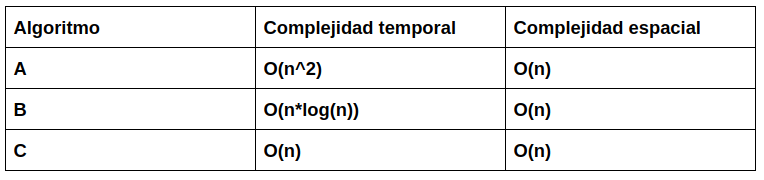
\includegraphics[width=\linewidth]{comparacion.png}
\end{figure}


Como se ve en la tabla, aunque todos tengan la misma complejidad espacial, el Algoritmo C supera a los demás, ya que es óptimo temporalmente.



\end{document}